\newpage
\chapter{Anordnung der Transistoren und Widerst�nde}
Das zu simulierende Modell  wurde daraufhin vereinfacht, dass die einzelnen Bauelemente durch Quader Repr�sentiert werden. Des weiteren wurde auf die Erstellung der Leiterbahnen verzichtet. Dadurch ergibt sich, dass die Leiterplatte ebenfalls durch einen einfachen Quader erstellt wird. Des Weiteren ist bei der Positionierung darauf zu achten, dass die abst�nde zwischen den Bauelementen in X-Richtung und in Y-Richtung Gleich gro� ist und innerhalb der Optimierung symmetrisch erweitert und verringert wird. 

\section{Transistoranordnung}
	Die Abbildung \ref{fig:Abmessungen_sot23} zeigt die Abmessungen eines Transistors der geforderten Bauform SOT23. Der Quader, welcher einen solchen Baustein repr�sentieren soll, erh�lt die darauf beruhenden Abmessungen h=1,1mm b=1,4mm h=3,0mm.
	\begin{center}
		\begin{minipage}[!ht]{0.8\textwidth}
			\captionsetup{type=figure}
			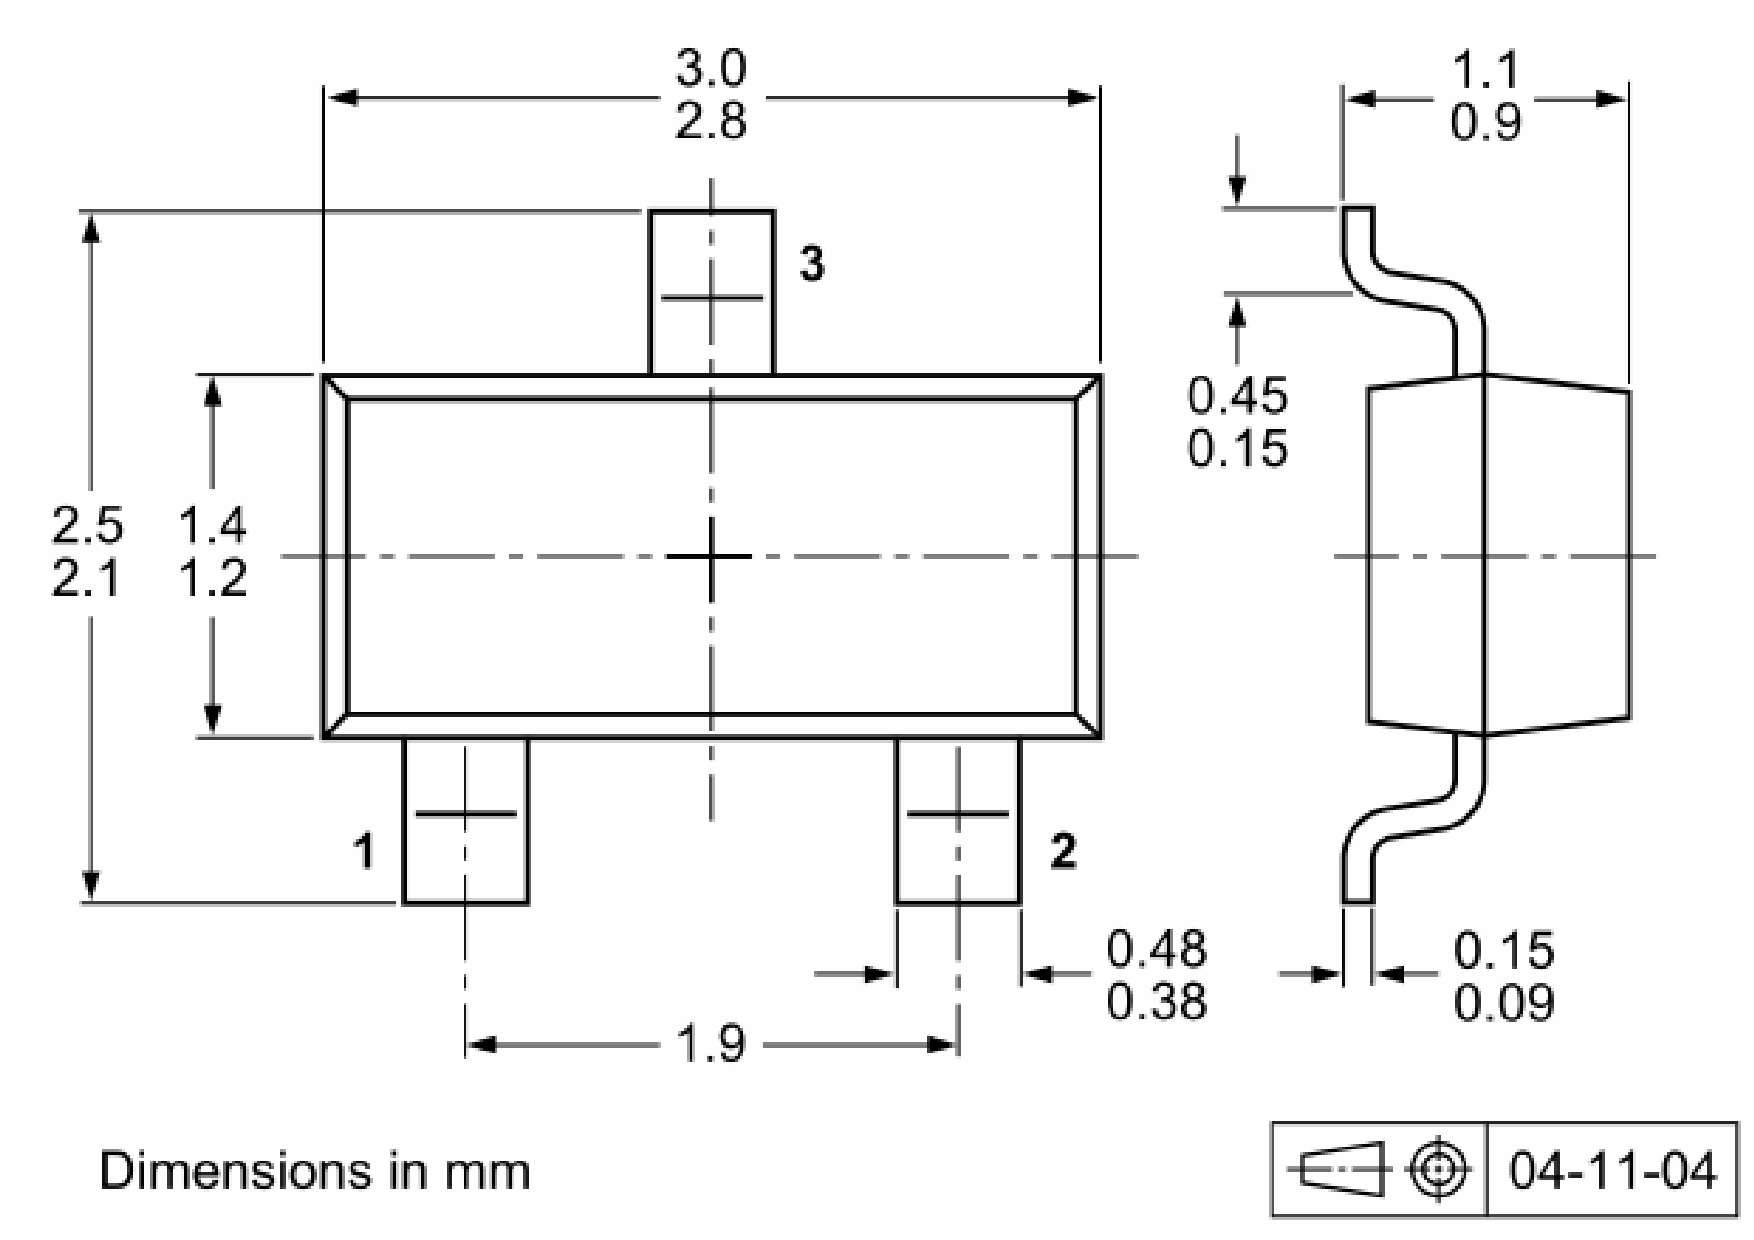
\includegraphics[width=1\linewidth]{bilder/Abmessungen_SOT23}
			\caption{Transistor - Abmessungen eines SOT23 Geh�uses, Quelle: NXP - PDTC114E Datenblatt S.10}
			\label{fig:Abmessungen_sot23}
		\end{minipage}
	\end{center}
	Um die Transistoren zu Positionieren, muss die Gr��e der Anschl�sse ber�cksichtigt werden. diese wiederum werden �ber die footprints ermittelt. (vgl. Abbildung \ref{fig:footprint_sot23} ) Somit ergibt sich ein Mindestabstand zwischen den Transistoren in Y-Richtung von 3 mm und in X-Richtung von 3,3 mm. Um nunmehr die Abst�nde synchron zu halten werden die Abst�nde in X-Richtung um weitere 1,6 mm Vergr��ert. Schlussendlich ergeben sich folgende Mindestabst�nde bzw. Vorgabelabst�nde:  
	\begin{table}[bh]
		\centering
		\caption{Abst�nde zwischen den Transistoren}
		\begin{tabular}{l >{\centering\arraybackslash}p{4cm} >{\centering\arraybackslash}p{4cm} } 
			\rowcolor[gray]{.8} & Y-Richtung & X-Richtung\\
			Mindestabstand = 0 mm& 4,6 mm & 3,3 mm\\	
			\rowcolor[gray]{.8}Sollabstand = 2 mm& 6,6 mm & 5,3 mm\\
		\end{tabular}
		\label{tab:Abst�nde SOT23}
	\end{table}
	
\section{Dimensionierung der Widerst�nde}
	
	\begin{center}
		\begin{minipage}[!ht]{0.8\textwidth}
			\captionsetup{type=figure}
			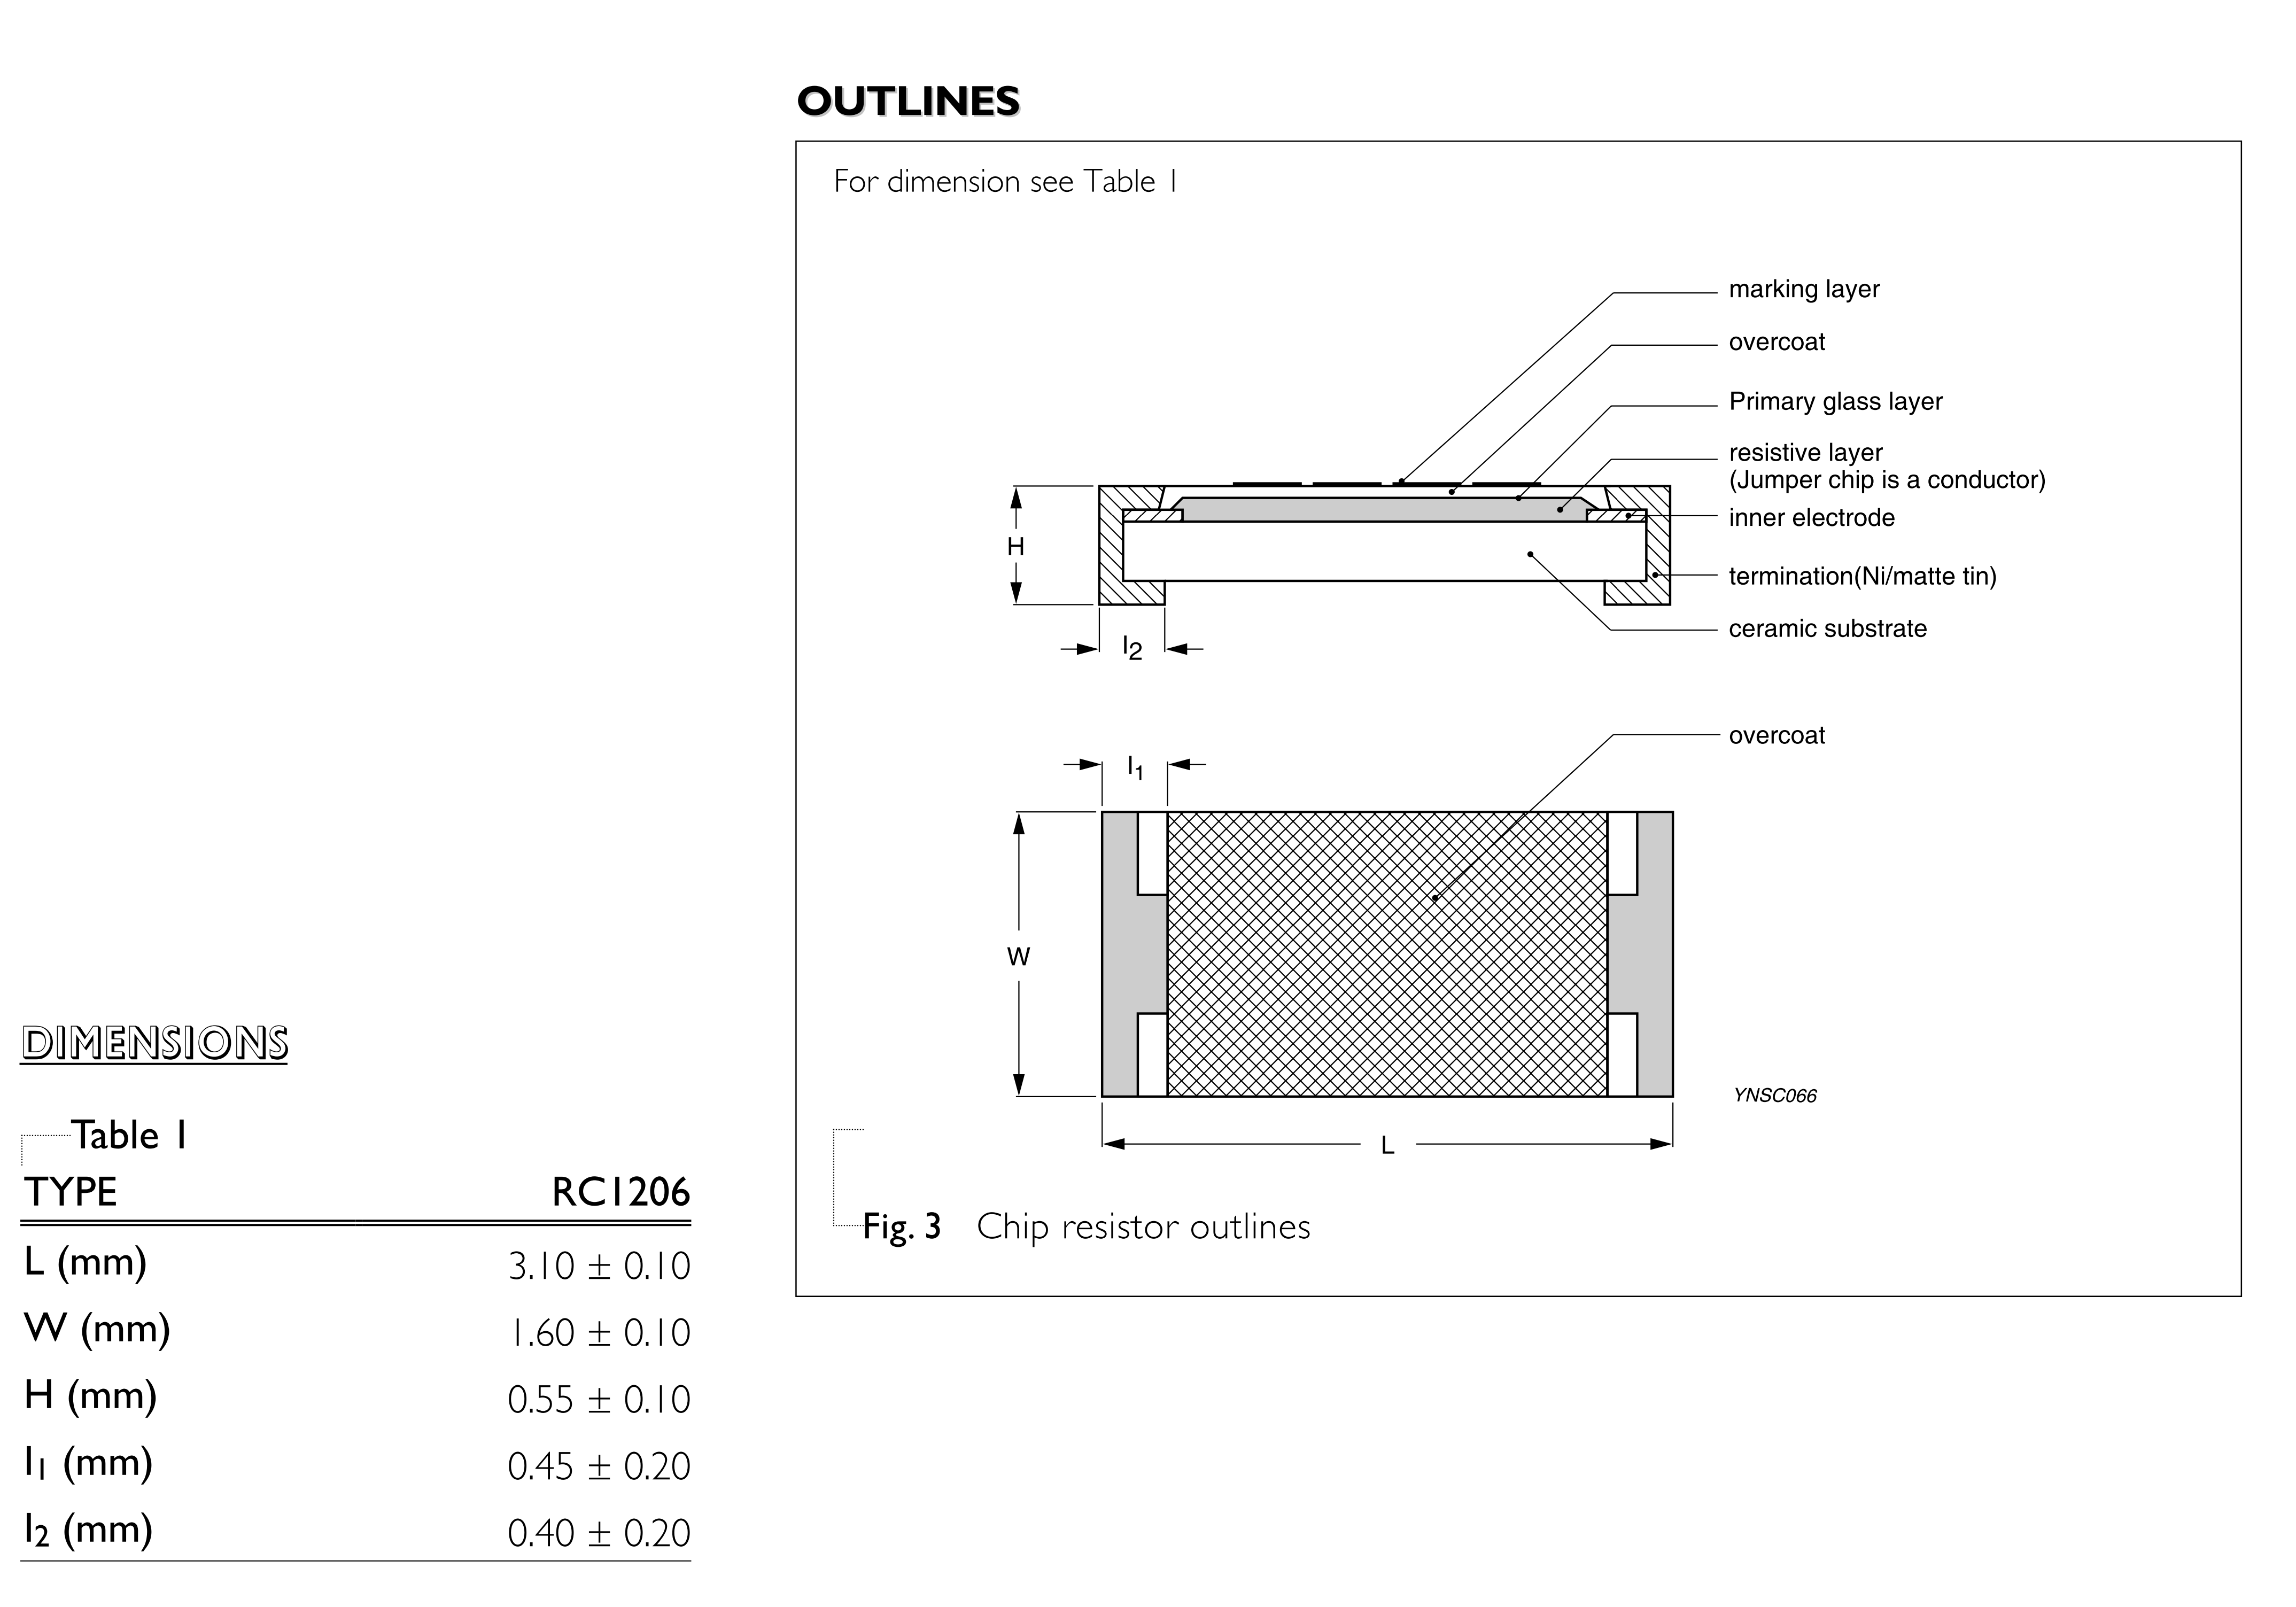
\includegraphics[width=1\linewidth]{bilder/Abnessungen_SMD_1206}
			\caption{Widerstand - Abmessungen SMD 1206, Quelle: Datenblatt RC1206 S.4}
			\label{fig:Abmessungen_SMD_1206}
		\end{minipage}
	\end{center}